\chapter{Decidability Problems for Hinged Polygons and Disks}
\section{The Logic Engine}
The \textit{logic engine} is a planar, mechanical device that simulates an instance NAE3SAT problem. It was introduced in \cite{BC87}.
\subsection{Construction of the Logic Engine}

\begin{figure}[!h]
\begin{center}
\includegraphics{graphics/LogicEngineFrameFigure1Scaled.pdf}
\caption{A logic engine frame with veritical armatures and a horizontal shaft.}
\label{fig:LogicEngineFrameFigure1.pdf}
\end{center}
\end{figure}

For a given a boolean formula, $\Phi$, in 3-CNF with $n$ variables and $m$ clauses, we construct a logic engine. The logic engine has a \textit{rigid frame} which houses the mechanical components of the the logic engine.  The rigid frame is the boundary of which the logic engine can operate within.  The 
\textit{shaft} is a horizontal line segment that is placed at mid-height of the rigid frame. The 
\textit{armatures} are veritical line segments whose midpoints are on the shaft.  Each armature 
has two orientations with respect to the shaft. 

\begin{figure}[!h]
\begin{center}
\includegraphics{graphics/LogicEngineFrameFigure1halfScaled.pdf}
\caption{A logic engine that corresponds to a boolean formula in NAE3SAT form, $\Phi$.  The picture shows the outer rigid frame, the shaft, the armatures that correspond to the variables in $\Phi$, with oriented flags.}\label{fig:LogicEngineFrameFigure1halfScaled.pdf}
\end{center}
\end{figure}

  Each armature corresponds to a variable in $\Phi$. There are two literals for each variable, i.e. 
the negated literal $\bar{x}_j$ and non-negated literal $x_j$.   Flagging arragement indicates the relationship of the boolean literal's existence within a clause.  Partition each armature into $2m$ unit, vertical line segments. Label the segments on the $j^\text{th}$ armature starting from the shaft by $\ell_{j,1},\ldots,\ell_{j,n}$ on one side and  $\bar{\ell}_{j,1},\ldots,\bar{\ell}_{j,n}$ on the other side of the shaft.  Attach regular triangles, called \textit{flags}, to some of these segments. Each segment is either flagged one or zero flags, i.e. \textit{flagged} or \textit{unflagged}. 

\begin{enumerate}
 \item If the literal $x_j$ is found in clause $C_k$, then $\ell_{j,k}$ is unflagged.
 \item If the literal $\bar{x}_j$ is found in clause $C_k$, then $\bar{l}_{j,k}$ is unflagged.
\end{enumerate}

Each flag has two orientations with respect to armature it is attached to.  Each flag has four potential positions, the flag can reflect left or right about the armature and the armature can reflect up or down about the shaft.
\begin{figure}[!h]
\begin{center}
\includegraphics{graphics/LogicEngineFrameFigure2Scaled.pdf}
\caption{A logic engine constructed from the boolean formula $\Phi = C_1 \cap C_2 \cap C_3$.}
\label{fig:LogicEngineFrameFigure2Scaled.pdf}
\end{center}
\end{figure}
The \textit{flags} are equilateral triangles
attached to the armatures.  The placement of the flags is dependent on the instance of the NAE3SAT 
boolean formula. Each flag as two orientations. 

For the NP hardness reduction in Theorem \ref{thm:LogicEngineV3-2} we need to make sure that all parameters in the logic engine can be specified polynomially in terms of the size of the boolean formula. Given $\Phi$, the corresponding logic engine is constructed as follows: all components will be specified with a 
quantity and coordinates defined as polynomials in $m$ and $n$.

\begin{center}
	\begin{table}\label{LogicEngineV3PolynomialTable}
		\begin{tabular}{|c|c|c|}%
			\hline
			Component & Quantity &  Set Definition\\ \hline
			Rigid Frame&1&$\set{(x,y)\in\bbr^2}{ \text{The boundary of }\left[ \frac{1}{2} , n + \frac{1}{2}\right] \times \left[ -m, m \right]}$\\ \hline
			Shaft&1&$\set{(x,y) \in \bbr^2}{x \in \left[\frac{1}{2}, n + \frac{1}{2}\right] \text{ and } y=0 }$\\ \hline
			Armatures & n & For the $j^\text{th}$ armature we have $\set{(x,y)\in\bbr^2}{x = j \text{ and } y \in [-m,m] }$\\ \hline
			Flags&$2mn-3m$& if $\ell_{j,k}$ is flagged then the attached flag is a regular triangle with side length 1.\\ \hline
		\end{tabular}
	\caption{The quantity and coordinates of the logic engine components.}
	\end{table}
\end{center}

\subsection{The mechanics of the logic engine}
A \textit{collision} of flags occur if either of the following occurs:
\begin{enumerate}
\item flags in the same row on adjacent armatures point toward each other.
\item a flag from the outermost armature $A_n$ points towards the outer rigid frame.
\item a flag from the innermost armature $A_1$ points inwards of $A_1$.
\end{enumerate}

\begin{figure}[!htbp]
\begin{center}
\includegraphics{graphics/logicEngineCollisions.pdf}
\caption{(a) Illustrates a adjacent flag collision at the same height, (b) and (c) illustrates a 
rigid frame collision.}\label{fig:logicEngineCollisions.pdf}
\end{center}
\end{figure}
The logic engine representation corresponding to $\Phi$ is to be configured such that no 
horizontally adjacent flags collide and flags do not collide with the rigid frame. 
\begin{figure}[!htbp]
\begin{center}
\includegraphics{graphics/logicEngineValidConfigurations.pdf}
\caption{The following configuration of adjacent flags 
and flags that are adjacent to the rigid frame.}\label{fig:logicEngineValidConfigurations.pdf}
\end{center}
\end{figure}

\begin{lem}\label{lem:logicEngine1}A row has a collision-free configuration if and only if it has 
at least one unglagged armature. \end{lem}
\begin{proof}
% Suppose that the flag on armature $A_1$ is flagged.  If the flag is oriented left, then there 
% is a flag-frame collision.  If the flag is oriented to the right and if $A_2$ is flagged, then 
% $A_2$ must also be oriented to the right; otherwise will result in a flag-flag collision.  Now 
% suppose the $i^\text{th}$ armature's flag is oriented to the right.  $A_{i+1}$ is also oriented to 
% the right; otherwise will result in a flag-flag collision. By induction all flags will orient to 
% the right up to $n$.  Thus the $n^\text{th}$ flag will will collide with the rigid frame.

Suppose all armatures are flagged in a row.  The flag on armature $A_1$ must point to the 
right otherwise we result in a rigid frame collision.  $A_2$ must point to the right otherwise 
we result in a rigid frame collision.  Without loss of generality, $A_i$ and $A_{i+1}$ must 
point to the right in order to prevent an adjacent flag collision.  This implies that $A_n$ 
must also point to the right which results into a rigid frame collision.

A same argument holds with the argument beginning with the flag 
on the armature $A_n$ pointing to the left.  Thus there is no collision-free configuration with 
all armatures flagged.


Suppose there is an unflagged armature in a row.  Turn all flags towards the nearest unflagged 
armature.  If there are flags on $A_1$ and $A_n$, point toward the interior thus they do not 
collide with the rigid frame.  If there are flags on two consecutive armatures, they do not collide 
because the nearest unflagged armature cannot be between them.  Therefore the row has a 
collision-free configuration.
\end{proof}

A logic engine is said to be \textit{collision-free configurable} when every row has a collision-free configuration.
\begin{figure}[!ht]
\begin{center}
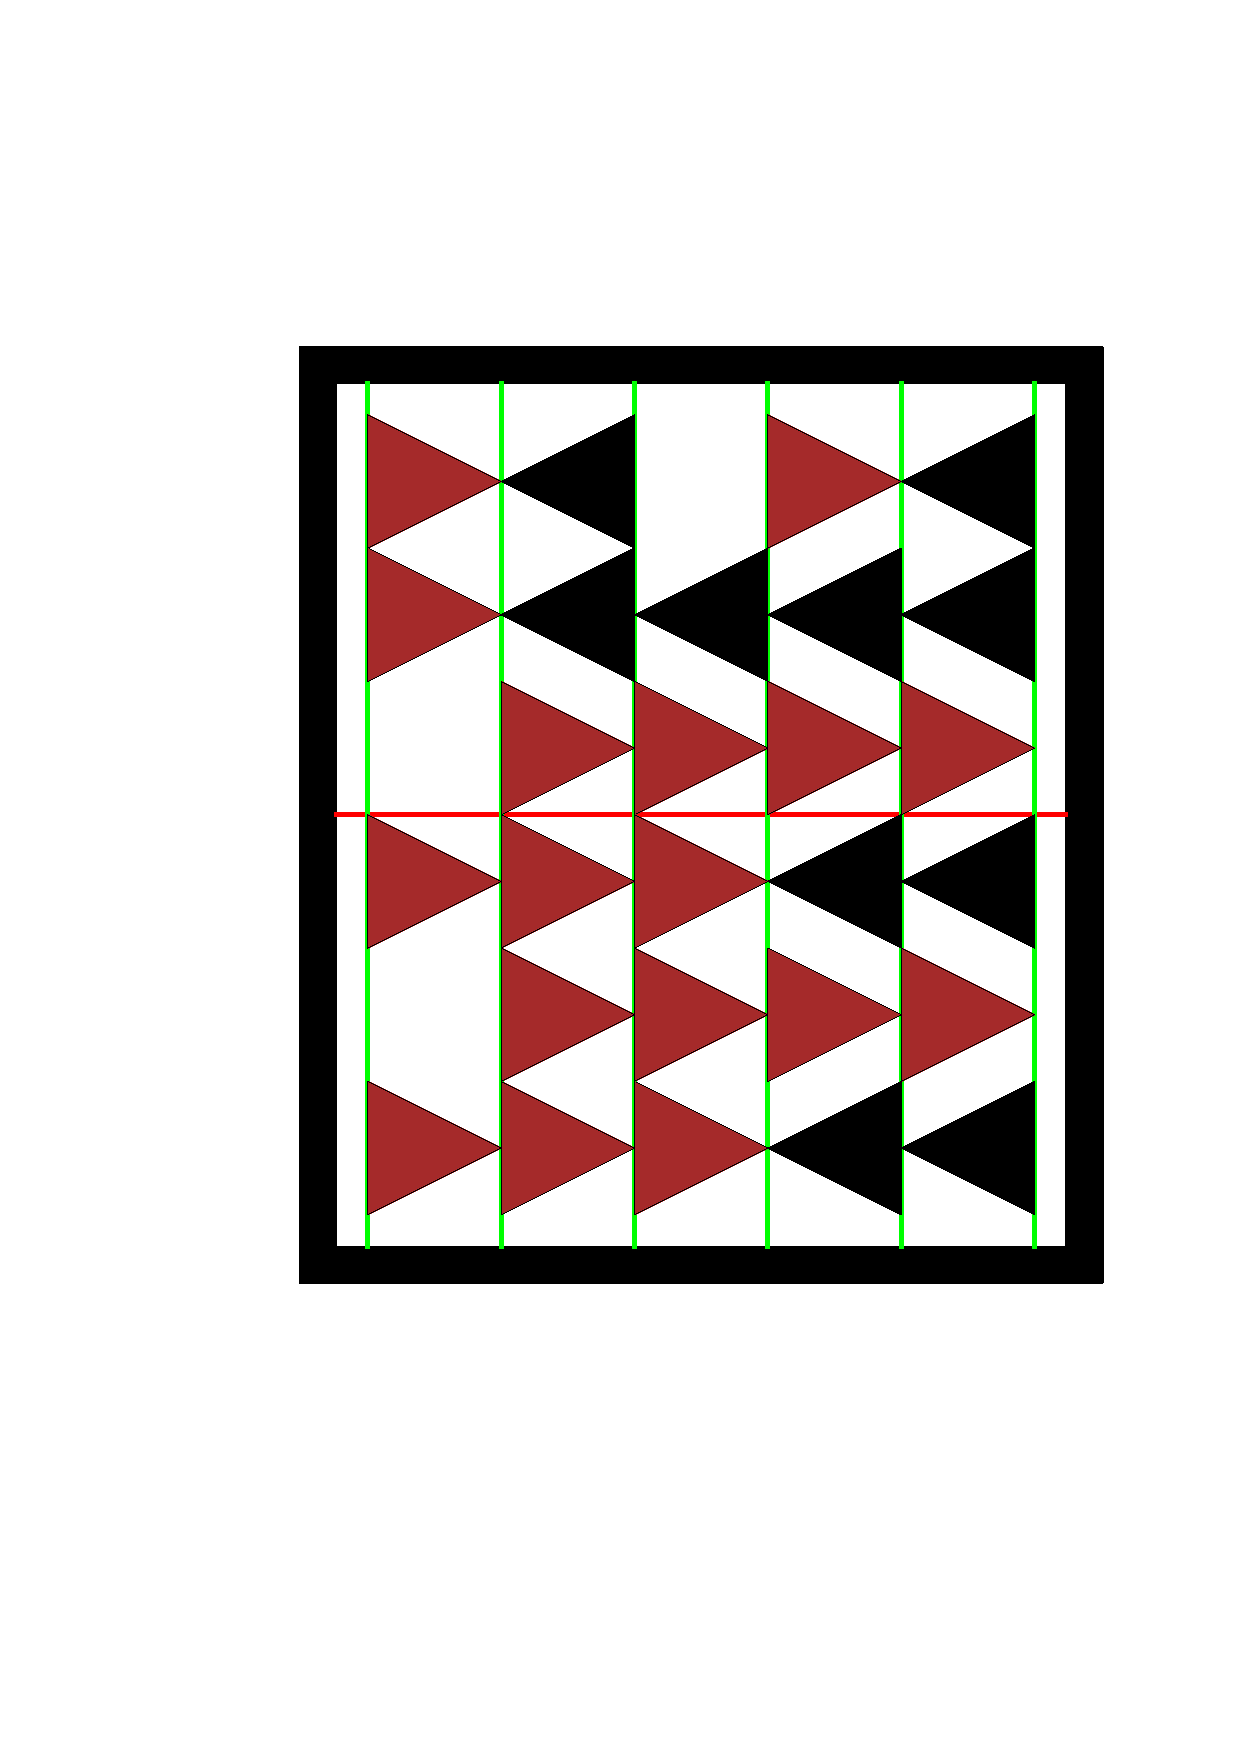
\includegraphics{graphics/LogicEngineFrameFigure5Scaled.pdf}
\caption{The logic engine from figure \ref{fig:LogicEngineFrameFigure2.pdf} whose armatures are rotated}\label{fig:LogicEngineFrameFigure5.pdf}
\end{center}
\end{figure}

\subsubsection{The Relationship of the Logic Engine and NAE3SAT}

We can show that given an boolean formula in 3-CNF form, $\Phi$, and a truth assignement, $\tau$, where the variables are given a truth assignment such that there is at least one true literal and one false literal in each clause of $\Phi$, then the corresponding logic engine to $\Phi$ is collision-free configurable.
\begin{thm}\label{thm:LogicEngineV3-1}
 Given an instance of a $NAE3SAT$,  it is a ``yes'' instance if and only if the corresponding logic 
engine is collision-free configurable.
\end{thm}
\begin{proof}
Suppose we have an instance of a $NAE3SAT$ that is a ``yes'' instance. This implies that there is a 
truth assignment such that each clause contains a true and a false literal. Now consider the logic 
engine corresponding to this instance. We now 
show that it has a collision free configuration.

For variables that are true, configure the armatures such that the flags corresponding to the 
non-negated literals reside above the 
shaft and the flags that correspond to the negated literals reside below this shaft.  For variables 
that are false, configure the 
armatures in the opposite orientation.  Each clause corresponds to a pair of rows in 
the logic engine, one row for non-negated literals and one for negated literals.  Because the 
$NAE3SAT$ is a yes instance, every row contains at least one unflagged armature.  
By Lemma \ref{lem:logicEngine1}, every row  has a collision-free configuration.

Suppose we have an instance of a $NAE3SAT$ such that the corresponding logic engine has a 
collision-free configuration. By Lemma \ref{lem:logicEngine1} every row at least one unflagged 
armature.  The $k^{th}$ clause is represented by the $k^{th}$ rows above and below the shaft. If the 
literal $x_j$ is found in clause $C_k$, then the armature is unflagged in that row. If the literal 
$\bar{x}_j$ is found in clause $C_k$, then $\bar{l}_{j,k}$ is unflagged.  All flags 
corresponding to negated literals reside below the shaft and flags corresponding to non-negated 
literals reside above the shaft.  All together we have that every clause has a true literal and a 
false literal.  Thus, we have a 'yes' instance of the $NAE3SAT$.
\end{proof}
\begin{thm}\label{thm:LogicEngineV3-2}
Deciding whether a logic engine is collision-free configurable is NP-Hard.
\end{thm}
\begin{proof}
In table \ref{LogicEngineV3PolynomialTable}, we defined the components of the logic engine in terms of polynomials in $m$ and $n$. If there were a polynomial time algorithm that decides whether a given logic engine is collision-free configurable, then by Theorem \ref{thm:LogicEngineV3-1} we would have a polynomial time algorithm to decide whether an instance of the NAE3SAT is a 'yes' instance.  Since NAE3SAT is NP-Hard \cite{NAE3SATisNPhard}, there is no such algorithm unless $P = NP$.
\end{proof}